\documentclass{standalone} 
\usepackage[tikz,plot,math]{forsyde}
\usepackage{forsyde-atom-docs}

\newcommand{\po}[1]{\underline{#1}}

\begin{document}
\begin{docimage}{example}
\begin{tikzpicture}[]
  \standard[process, moc=sdf, ni=2, no=2, f={$\lambda (a,b,c) (d,e) \rightarrow ((a+d,c+e),(b))$}, type=comb](p1){};
  \inputSY*[anchor=south west, shift={(-3cm, .2cm)}]  <p1.w1> {\po{1,2,3},\po{4,5,6},\po{7,8,9},...};
  \inputSY*[anchor=south west, shift={(-3cm,-.2cm)}]  <p1.w2> {\po{1,1},\po{1,1},\po{1,1},1};
  \outputSY*[yshift=.2cm]  <p1.e1> {\po{2,4},\po{5,7},\po{8,10}};
  \outputSY*[yshift=-.2cm]  <p1.e2> {\po{2},\po{5},\po{8}};
\end{tikzpicture}
\end{docimage}


\begin{docimage}{pattern-delay}
\begin{tikzpicture}[]
  \standard[process, moc=sdf, ni=1, no=1, f={$[0,0,0]$}, type=delay](p1){};
  \inputSY*  <p1.w1> {1,2,3,4,5};
  \outputSY*  <p1.e1> {0,0,0,1,2,3,4,5};
\end{tikzpicture}
\end{docimage} 

\begin{docimage}{pattern-delayp}
\begin{tikzpicture}[]
  \standard[process, moc=sdf, ni=2, no=1, type=delay'](p1){};
  \inputSY*[anchor=south west, shift={(-2cm, .2cm)}]  <p1.w1> {1,2,3,4,5};
  \inputSY*[anchor=south west, shift={(-2cm,-.2cm)}]  <p1.w2> {0,0,0};
  \outputSY*[]  <p1.e1> {0,0,0,1,2,3,4,5};
\end{tikzpicture}
\end{docimage} 

\begin{docimage}{pattern-comb}
\begin{tikzpicture}[]
  \standard[process, moc=sdf, ni=2, no=1, f={$\lambda (a,b,c) (d,e) \rightarrow ((a+d,c+e),(b))$}, type=comb](p1){};
  \inputSY*[anchor=south west, shift={(-2cm, .2cm)}]  <p1.w1> {\po{1,2,3},\po{4,5,6},\po{7,8,9},...};
  \inputSY*[anchor=south west, shift={(-2cm,-.2cm)}]  <p1.w2> {\po{1,1},\po{1,1},\po{1,1},1};
  \outputSY*[]  <p1.e1> {\po{2,4},\po{5,7},\po{8,10}};
\end{tikzpicture}
\end{docimage} 

\begin{docimage}{pattern-constant}
\begin{tikzpicture}[]
  \standard[process, moc=sdf, no=2, f={$((1,2,3),(2,1))$}, type=constant](p1){};
  \outputSY*[yshift=.2cm]  <p1.e1> {\po{1,2,3},\po{1,2,3},...};
  \outputSY*[yshift=-.2cm] <p1.e2> {\po{2,1},\po{2,1},\po{2,1},...};
\end{tikzpicture}
\end{docimage} 

\begin{docimage}{pattern-generate}
\begin{tikzpicture}[]
  \standard[process, moc=sdf, no=2,
    f={$\lambda\ a\ b \rightarrow ((\Sigma a, \Sigma a),(\Sigma b, \Sigma b, \Sigma b))$;$(1,1),(2,2,2)$},
    type=generate](p1){};
  \outputSY*[yshift=.2cm]  <p1.e1> {\po{1,1},\po{2,2},\po{4,4},8,...};
  \outputSY*[yshift=-.2cm] <p1.e2> {\po{2,2,2},\po{6,6,6},18,18,...};
\end{tikzpicture}
\end{docimage} 

\begin{docimage}{pattern-state}
\begin{tikzpicture}[]
  \standard[process, moc=sdf, f={$\lambda(a)(b,c) \rightarrow (a+b+c)$;$(1)$}, type=state](p1){};
  \inputSY*  <p1.west> {\po{1,2},\po{3,4},\po{5,6},7};
  \outputSY* <p1.east> {\po{1},\po{4},\po{11},\po{22}};
\end{tikzpicture}
\end{docimage} 

\begin{docimage}{pattern-stated}
\begin{tikzpicture}[]
  \standard[process, moc=sdf, f={$\lambda(a)(b,c) \rightarrow (a+b+c)$;$(1)$}, type=stated](p1){};
  \inputSY*  <p1.west> {\po{1,2},\po{3,4},\po{5,6},7};
  \outputSY* <p1.east> {\po{4},\po{11},\po{22}};
\end{tikzpicture}
\end{docimage}

\begin{docimage}{pattern-moore}
\begin{tikzpicture}[]
  \standard[process, moc=sdf, f={$\lambda(a)(b,c) \rightarrow (a+b+c)$;$\lambda(a) \rightarrow (a+1,a\times 2)$;$(1)$}, type=moore](p1){};
  \inputSY*  <p1.west> {\po{1,2},\po{3,4},\po{5,6},7};
  \outputSY* <p1.east> {\po{2,2},\po{5,8},\po{12,22},\po{23,44}};
\end{tikzpicture}
\end{docimage}

\begin{docimage}{pattern-mealy}
\begin{tikzpicture}[]
  \standard[process, moc=sdf, f={$\lambda(a)(b,c) \rightarrow (a+b+c)$;$\lambda(a)(b) \rightarrow (a+b,a\times b)$;$(1)$}, type=mealy](p1){};
  \inputSY*  <p1.west> {\po{\po{1},\po{2}},\po{\po{3},4},\po{5,6},7};
  \outputSY* <p1.east> {\po{2,1},\po{6,8},\po{14,33},\po{26,88}};
\end{tikzpicture}
\end{docimage}

\begin{docimage}{tosy}
\begin{tikzpicture}[]
  \standard[process, ni=1, moc=sdf, type=toSY](p1){};
  \inputSY*  <p1.w1> {1,2,3,4,5};
  \outputSY* <p1.e1> {1,2,3,4,5};
\end{tikzpicture}
\end{docimage}


\end{document}

%%% Local Variables:
%%% TeX-command-default: "Make"
%%% mode: latex
%%% TeX-master: t
%%% End:
